\documentclass[a4paper,10pt]{article}
\usepackage[utf8]{inputenc}
\usepackage{graphicx} 

\begin{document}

\begin{titlepage}
    \centering
        {\bfseries\Large
        Kaggle Titanic competition\\
        March 2015
        
    }  
     \vfill
     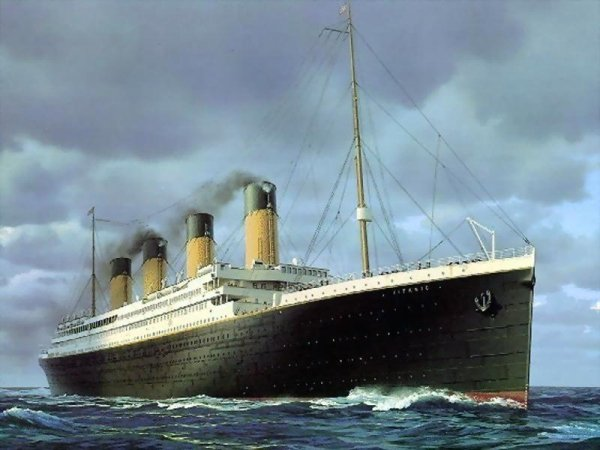
\includegraphics[width=10cm]{titanic.jpg} % also works with logo.pdf
    \vfill
    {\bfseries\Large

        Hugo Braun, Nicolas Legroux (INF582\_90)\\
        \vskip2cm
        INF582
    }    
    \vfill
   
  
\end{titlepage}

\section{Introduction}
The Titanic Kaggle competition defines a data science challenge : by using some features concerning the passengers onboard the Titanic (Name, Age, Family characteristics...), and a train dataset, we have to predict if a passenger has died during the sinking. \\

To solve the problem, we tried different approaches, by using various classifiers and performing feature engineering. Our best score on the Kaggle leaderboard was 0.82297 (with username INF582\_90), which was obtained after some work in engineering features and by using a Random Forest.

\section{Feature cleaning and engineering phase}

\subsection{Feature Cleaning}

The first thing we did was to clean up the data, using the Pandas python library. \\

In the few cases where the Fare or the Embarcation port was missing, we replaced the missing values with, respectively, the median fare (after taking into account the Class of the passenger) and 'Southampton', where most of the passengers embarked on the ship. \\

Some columns simply had too much missing data to try to effectively guess the missing values. This is for example the case with the Cabin column. Nevertheless we did not drop any column from the start and used pretty much all the columns in feature engineering as we will see in the next section. \\

The tricky column is the 'Age' column: about 30\% of the data is missing. At first, we replaced the missing values by computing medians for each ('Sex', 'PClass') subset (we saw by plotting the data that on the Titanic, men were older than women and first-class passengers were older than third-class passengers). Later on, we refined this by replacing the 'Sex' feature with the 'Title' feature, which allowed us to discriminate between boys (who have the Title 'Master') and older men (who have the Title 'Mr'), as well as between unmarried women ('Miss') and married women ('Mrs').

\subsection{Feature engineering : Titles, Family groups, Dummy variables}

Most of the work was focussed on feature engineering, as we saw that this is what really allowed to improve our scores. \\

Our first engineered feature was to extract the Title from the passenger Name. We only kept a set of four Titles : 'Mrs', Miss', 'Master', and 'Mr'. This is interesting since for example, most (56\%) of the "Masters" on the Titanic survived, whoch was not visible with only the 'Sex' variable. In fact, during the training stage, this new feature is always the one that is considered the most significant by the classifiers. \\

Even though a lot of Cabins were missing, we still extracted from that variable a Deck feature which we hoped might be interesting as it allowed us to separate some of the passengers according to where they were sleeping on the ship, which could prove signficant for survival. \\

We also identified Families and Groups on the ship. To identify families, we used the Name, Parch (number of parents or children) and SibSp (number of siblings or spouses) variables. To identify Groups (ie. people travelling together who are not necessarily in the same family), we used the Ticket variable (some people purchased their ticket together and therefore have the same ticket number). This last step allowed us, for example, to :

\begin{itemize}
\item Group maids with their families (quite a few fist-class families had maids travelling with them)
\item Identify a group of eight Third-Class men with Asian-sounding names who appeared to do quite well to survive (in the training set, the majority survived, which was very unlikely for third-class men). This gave us ideas as we will see later on.
\end{itemize}

Finally, we created dummy variables for most of the categorical features (like the Class, the Title, the Deck...) as the Python classifiers in the Sklearn library cannot really handle categorical features when there is no logical ordering of the feature values.

\subsection{Feature engineering : identifying outliers}

The features discussed in the previous section allowed us to reach 79\% on the Kaggle platform. We managed to improve the score by 3\% by adding two other features which we will now discuss. \\

The idea was the following: we thought that identifying outliers could prove significant in judging the survival of the Family or Group members of those outliers. We got this idea, in part by seeing the group of eight third-class men discussed above, and in part by simply considering that when a mother died on the Titanic, the rest of her family also probably died. \\

Simply grouping the families isn't enough as there are too many of them and using dummy variables for each family or group would be intractable. \\

Instead, we created two new binary features :

\begin{itemize}
\item The first identifies all passengers who have, in their Family or in their Group, an adult male passenger who survived. The idea is that it is very likely that these people survived (during the disaster, there was no chance that for example, a father would get on on a lifeboat before his children).
\item The second feature identifies all passengers who have, in their Family or Group, a women or a child who died. The idea is that it is very likely that in that case, the passenger died (this, for example, helps us predicting the death of a child when his mother did not survive).
\end{itemize}

Adding those two features allowed us to reach 82\% on the Kaggle leaderboard.

\section{Tools for the training phase}

\subsection{Evaluation with cross validation}

We implemented Cross validation in order to get some feedback about our models without using Kaggle. We used a Cross validation fold number equal to 10. Surprisingly, the results of Cross validation were always a few percentage points above the Kaggle ladder score, which has us wondering whether the train and test data were split randomly or whether this was just due to the low size of the data.

\subsection{Parameters optimisation}

In order to improve our classifiers we tried different methods. One of them was using the Sklearn capacities of RandomizedSearchCV. This function tries different parameters value in a predefined range and returns the most promising ones. Unfortunately, that method didn't really help us to get a better score.

\subsection{Learning curve}

In order to have control on the bias and variance of our classifiers we used learning curves. This helped us to notice the high variance of our Decision Trees and led us to use a Random Forest.

\begin{figure}[h!]
  \centering
    
      \includegraphics[width=10cm]{lurning_curve.png}
  \caption{Lurning curve}
\end{figure}


\section{Training phase}
\subsection{First Decision Tree}

We first started with a very simple decision tree. We limited its depth to 3, and we used only the features directly present
in the data. This decision scored 0.77 on Kaggle, which is just above the simple `Gender` approach, but allowed us to 
get into the problem. \\

The tree predicted well the 'easy' profiles, using the gender and class information. We now had to find a way to have a better fit on the harder cases.

\subsection{Adding new features (1/2)}

We then added features described in section 2.2.\\

We decided to use a Random Forest to use those new features. We were thinking that for instance the Surname feature would be useful only with a lot of weak classifiers. We got a score above 0.78 by using that forest. \\

We then tried to improve our use of those features : We merged different categorical values together (like Mme and Mrs, or 
all the superior titles like 'Capt', 'Dr', etc. into one : 'Mr'). We also created the dummy features described in 2.2.\\

All these modifications got us to slightly improve the score. We noticed in a DecisionTree (depth 3) that for instance the Deck E 
played a special role in the sinking.\\

We then used the 'GroupID' feature. The idea behind that feature is like the one for families : we presume that the people who were traveling together were at the same place when the accident occured. By using that feature, we managed
to get above the score of 0.79.

\subsection{Adding new features (2/2)}

Finally to get above 80\% we used the two features described in section 2.3. \\

Just after computing these features, we tried a very simple Decision Tree, of depth 2. The Decision Tree can be seen in Figure 2. \\

This very simple tree got us a score of 81.8\% on Kaggle.

 \newpage

\begin{figure}[h!]
  \centering 
    
      \includegraphics[width=10cm]{DecisionTree.png}
  \caption{Decision Tree with outliers}
\end{figure}

After this we managed to improve slightly our score, achieving 82.2\% on Kaggle with a Random Forest.


\subsection{Bagging}

To that point, we had only used trees or forests. We tried other classifiers, like Logistic Regression (with only dummy features -- logistic regression doesn't work with categorical features labeled with integers), and Ensemble methods like AdaBoost, GradientBoosting and Extra Trees. The idea is that a classifier can be better than an other one in a particular situation. To combine the result of all the classifiers used, we finally 
used a Decision Tree.

\begin{figure}[h!]
  \centering
    
      \includegraphics[width=13cm]{finalTree.png}
  \caption{Final decision tree}
\end{figure}

That method, unfortunately, didn't do better than the 82.2\% we got with the Random Forest.

\end{document}          
